The goal of our research is to develop an automatic way to detect design and requirement \SATD comments \emad{need to make sure this is consistent with the goal in the beg of section 2}. To do so, we first manually classify a large number of comments identifying which ones are \SATD. With the resulting dataset, we train the NLP tool to identify design and requirement \SATD (RQ1). To better understand what words indicate \SATD, we inspect the features used by the NLP tool to identify the detected technical debt. These features are words that are frequently found in comments with technical debt. We present the 10 most common words that indicate design and requirement \SATD (RQ2). Since the manual classification required to create our training dataset is expensive, ideally we would like to achieve maximum performance with the least amount of training data. Therefore, we investigate how variations in the size of training data affects the performance of our classification (RQ3). We detail the motivation, approach and present the results of each of our research questions in the remainder of this section.    

\begin{figure*}[!thb]
  \centering
  % \subfigure[Design Debt]{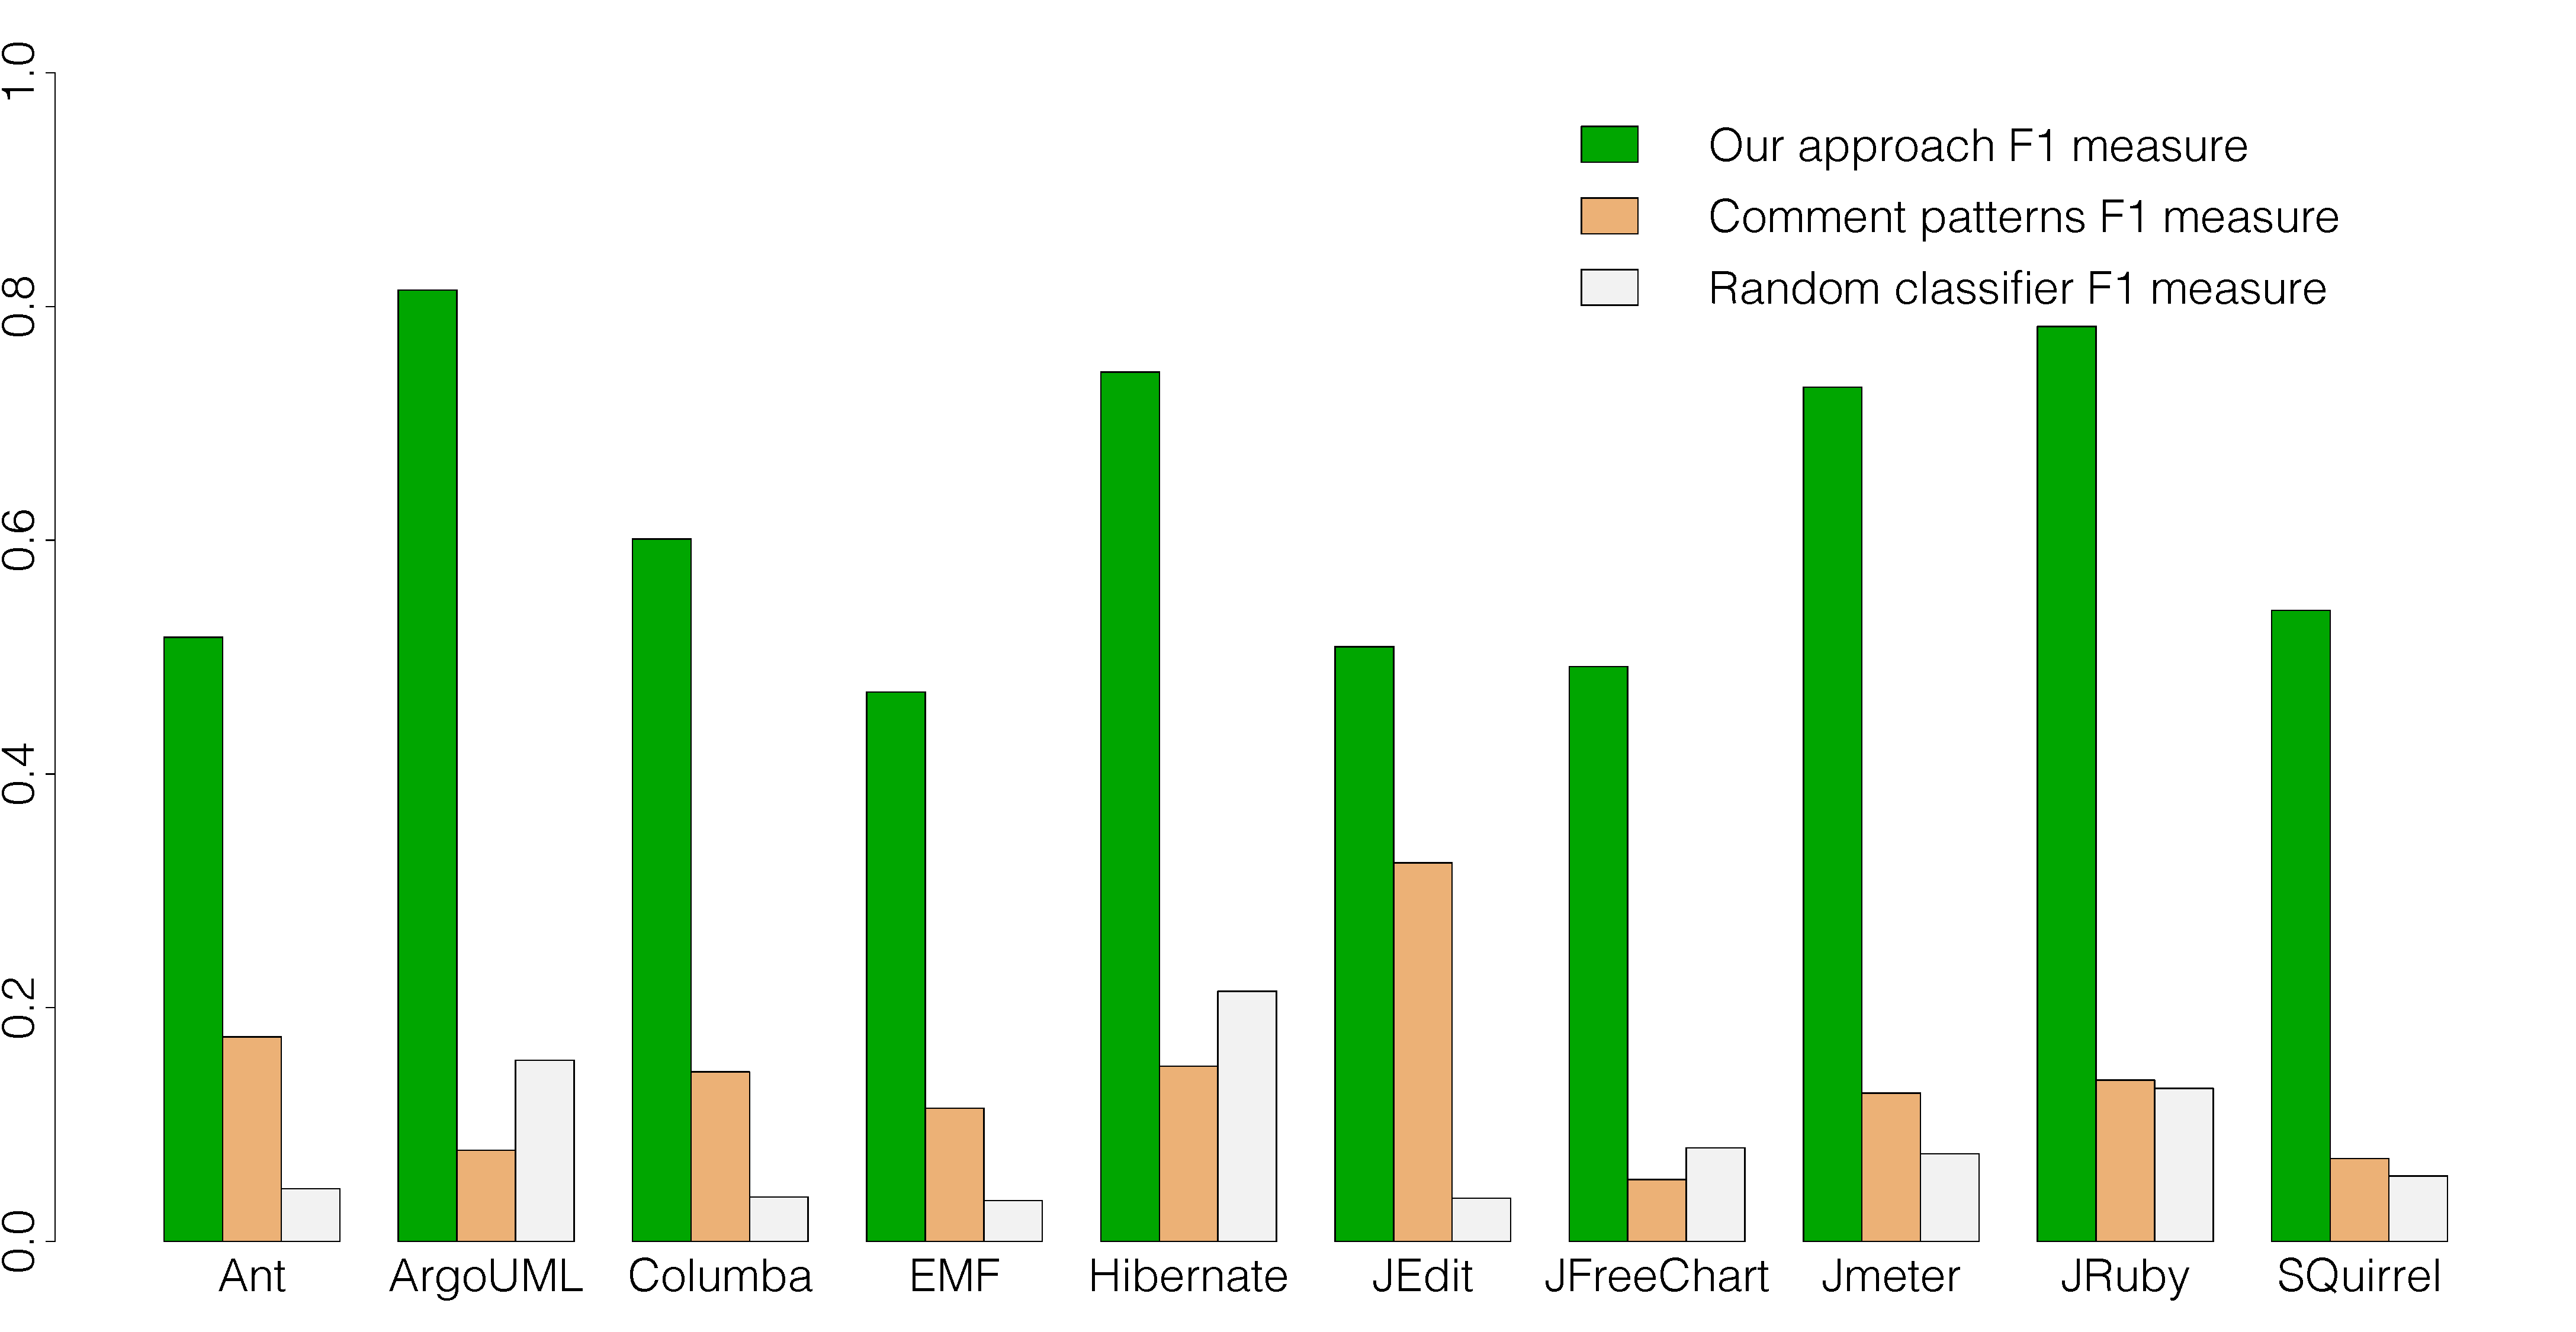
\includegraphics[width=0.48\textwidth]{figures/f1_measure_comparisom_design.pdf}
  \subfigure[Design Debt]{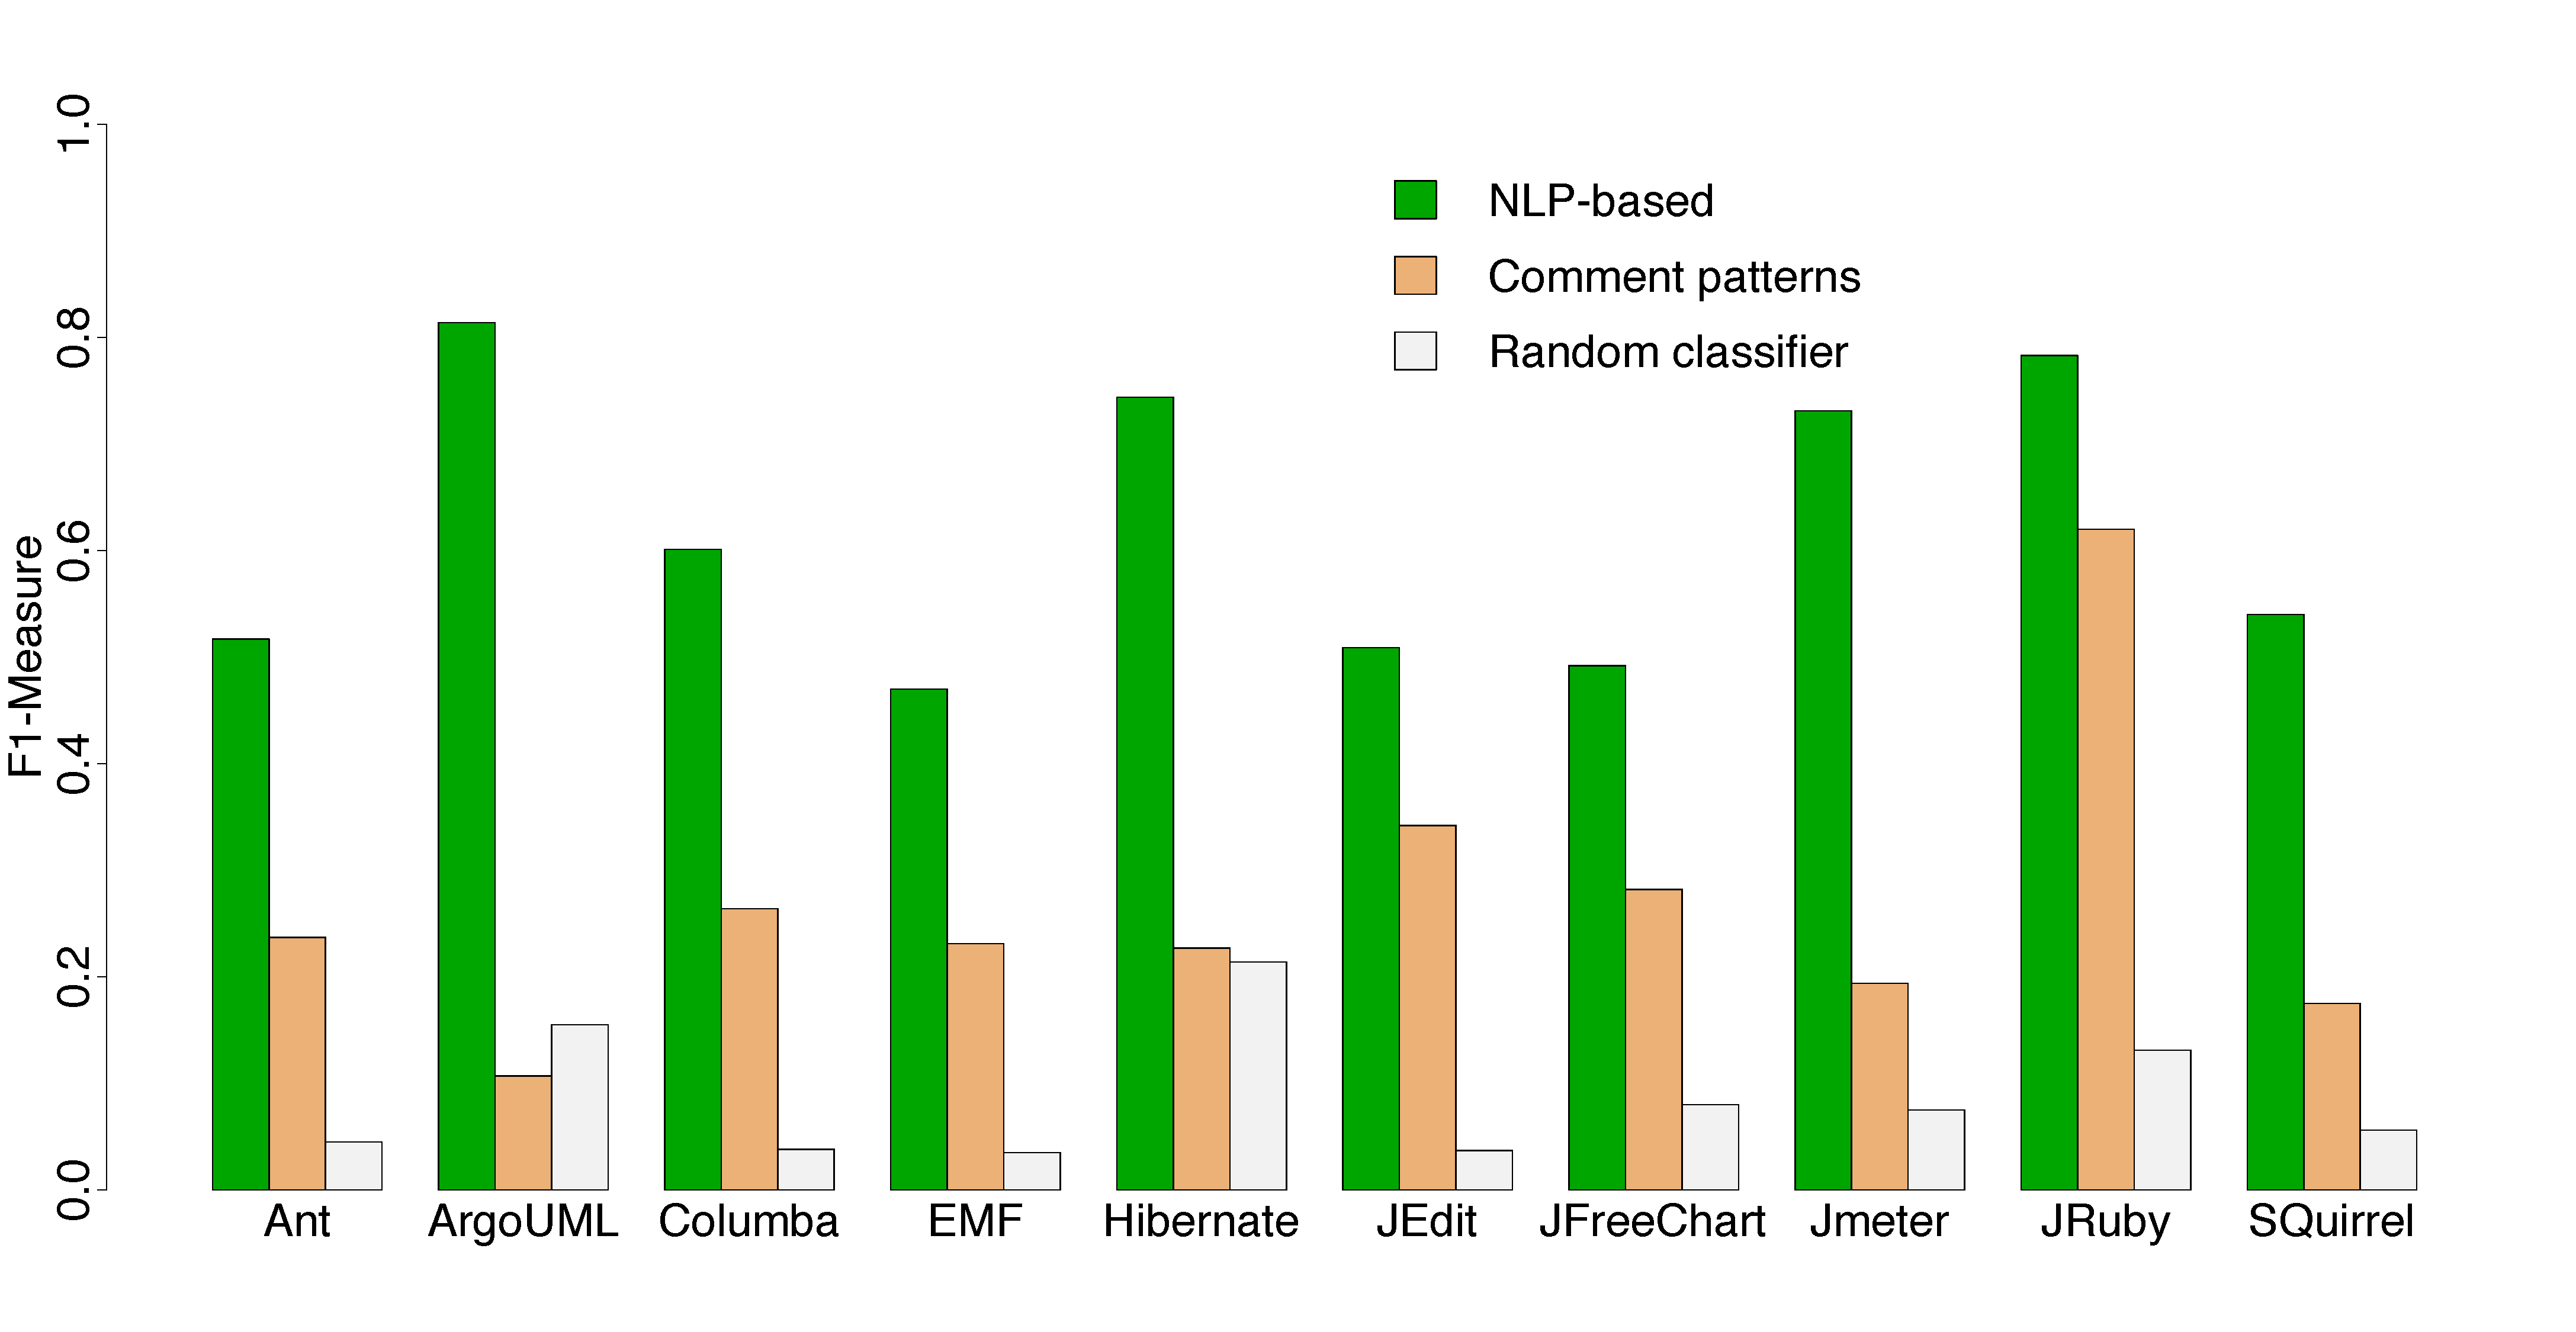
\includegraphics[width=0.49\textwidth]{figures/f1_measure_comparisom_design_1.pdf}
  \label{fig:f1_measure_comparison_design_debt}}
  % \subfigure[Requirement Debt]{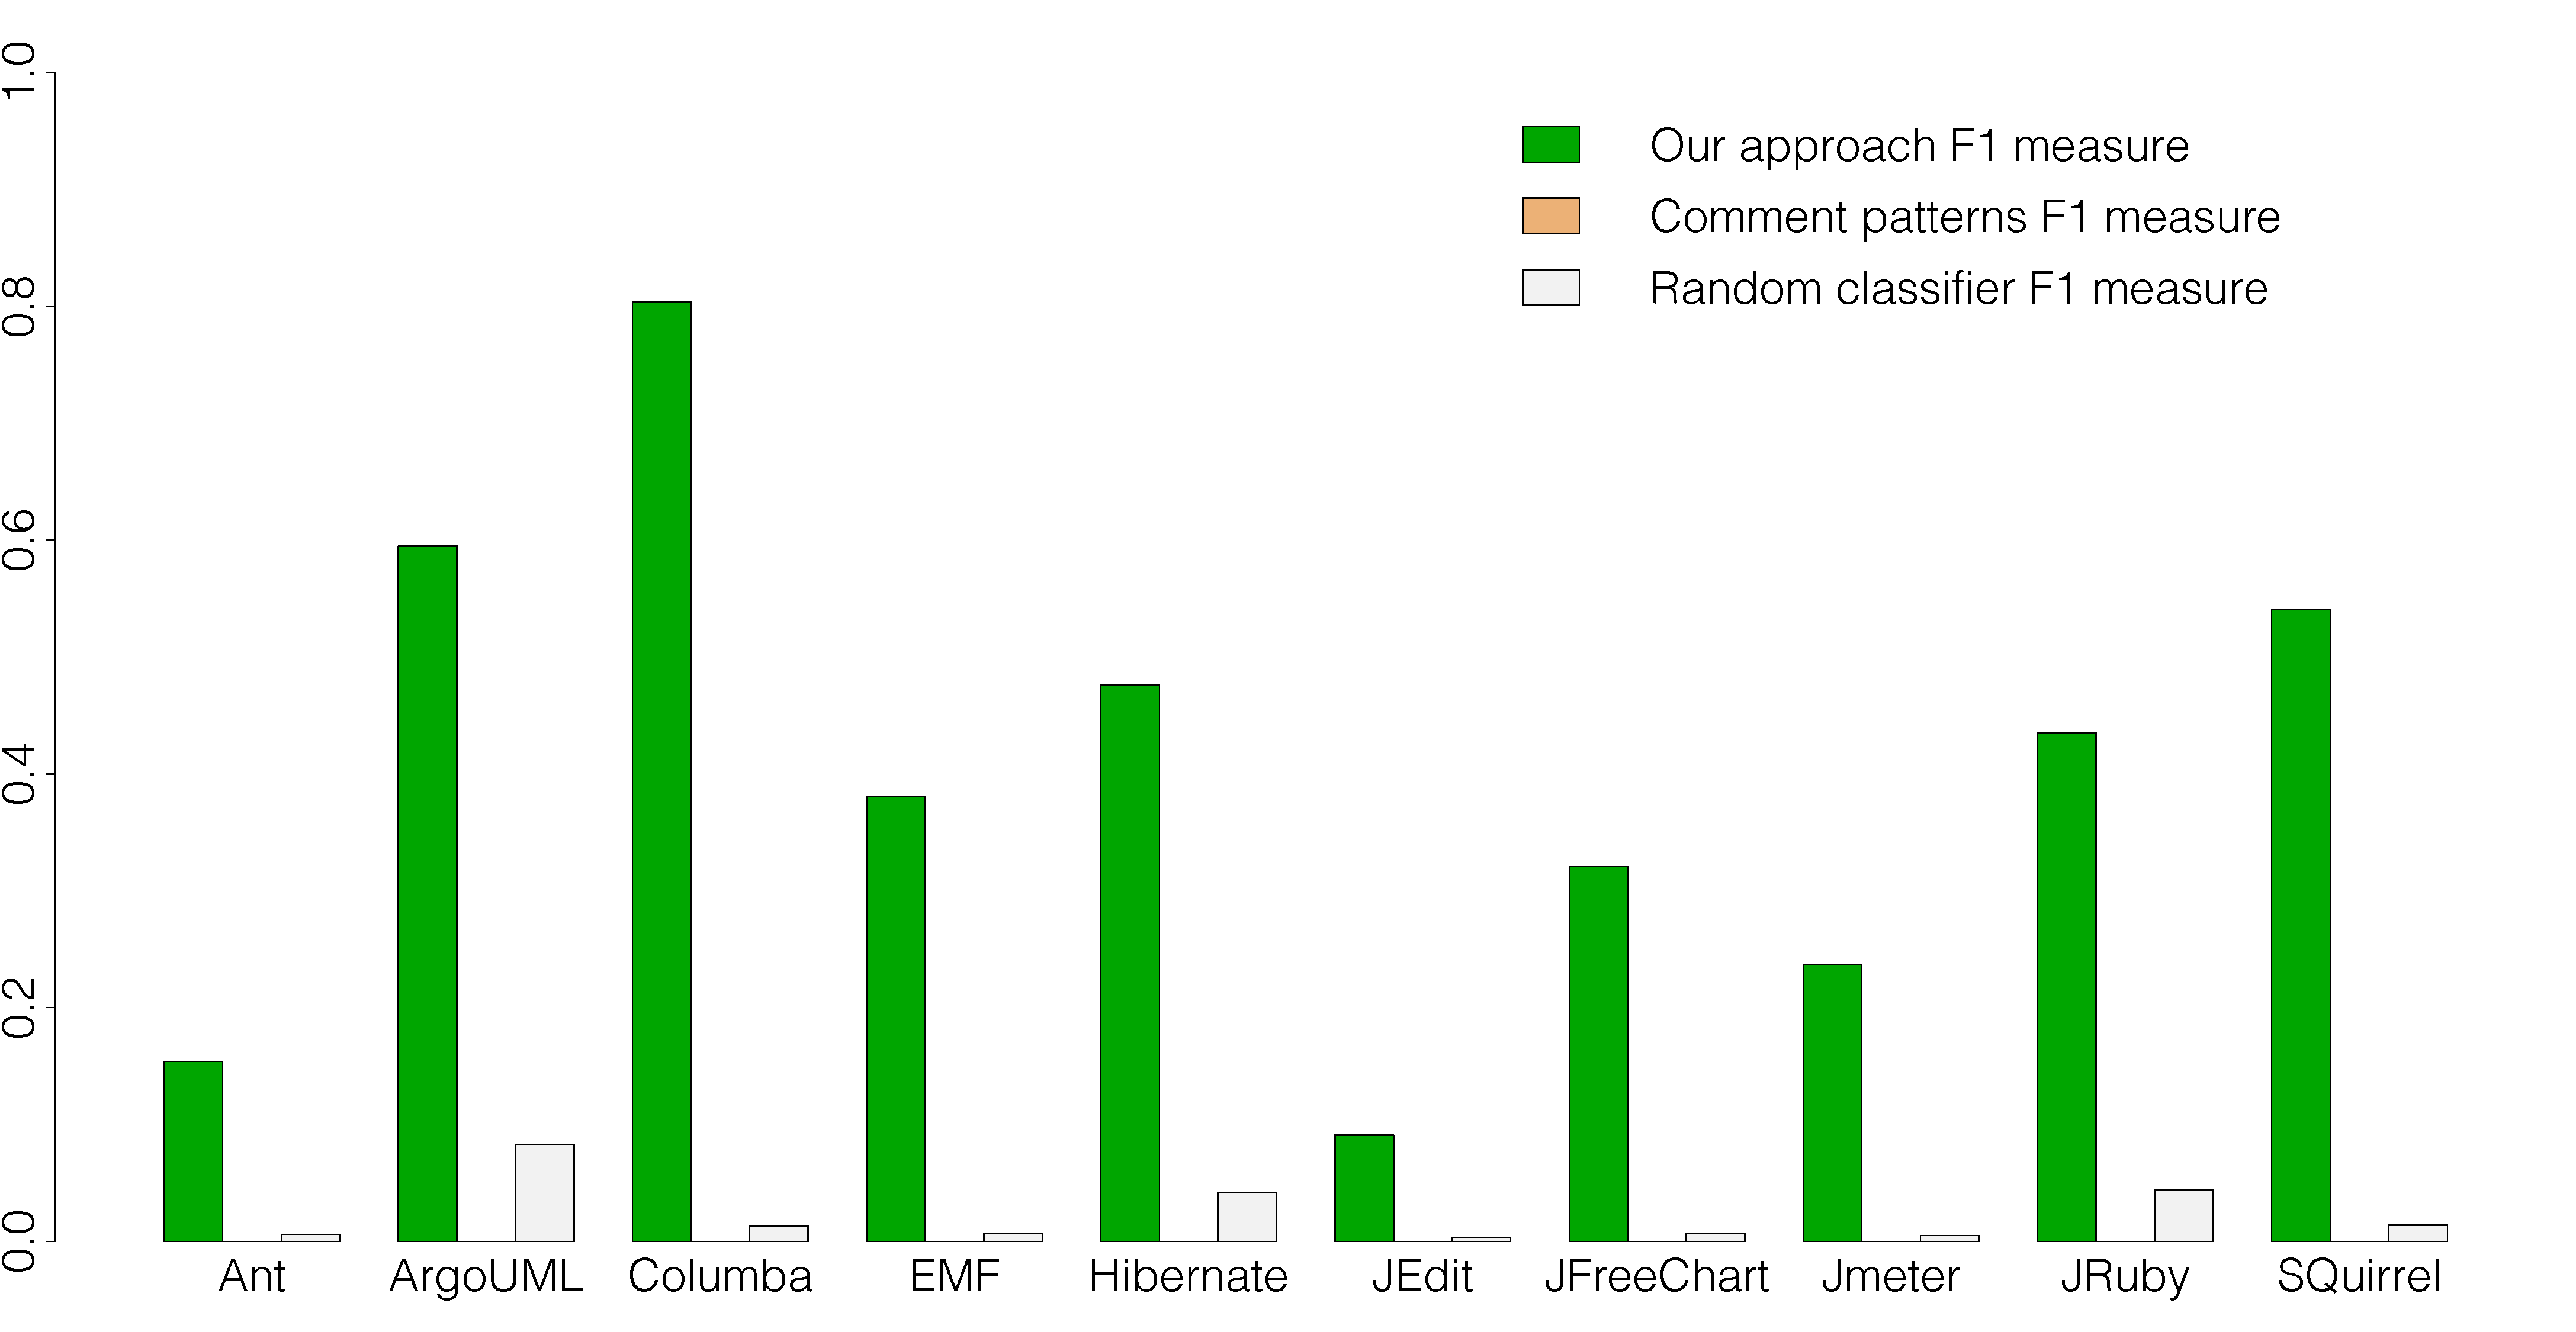
\includegraphics[width=0.48\textwidth]{figures/f1_measure_comparisom_requirement.pdf}
  \subfigure[Requirement Debt]{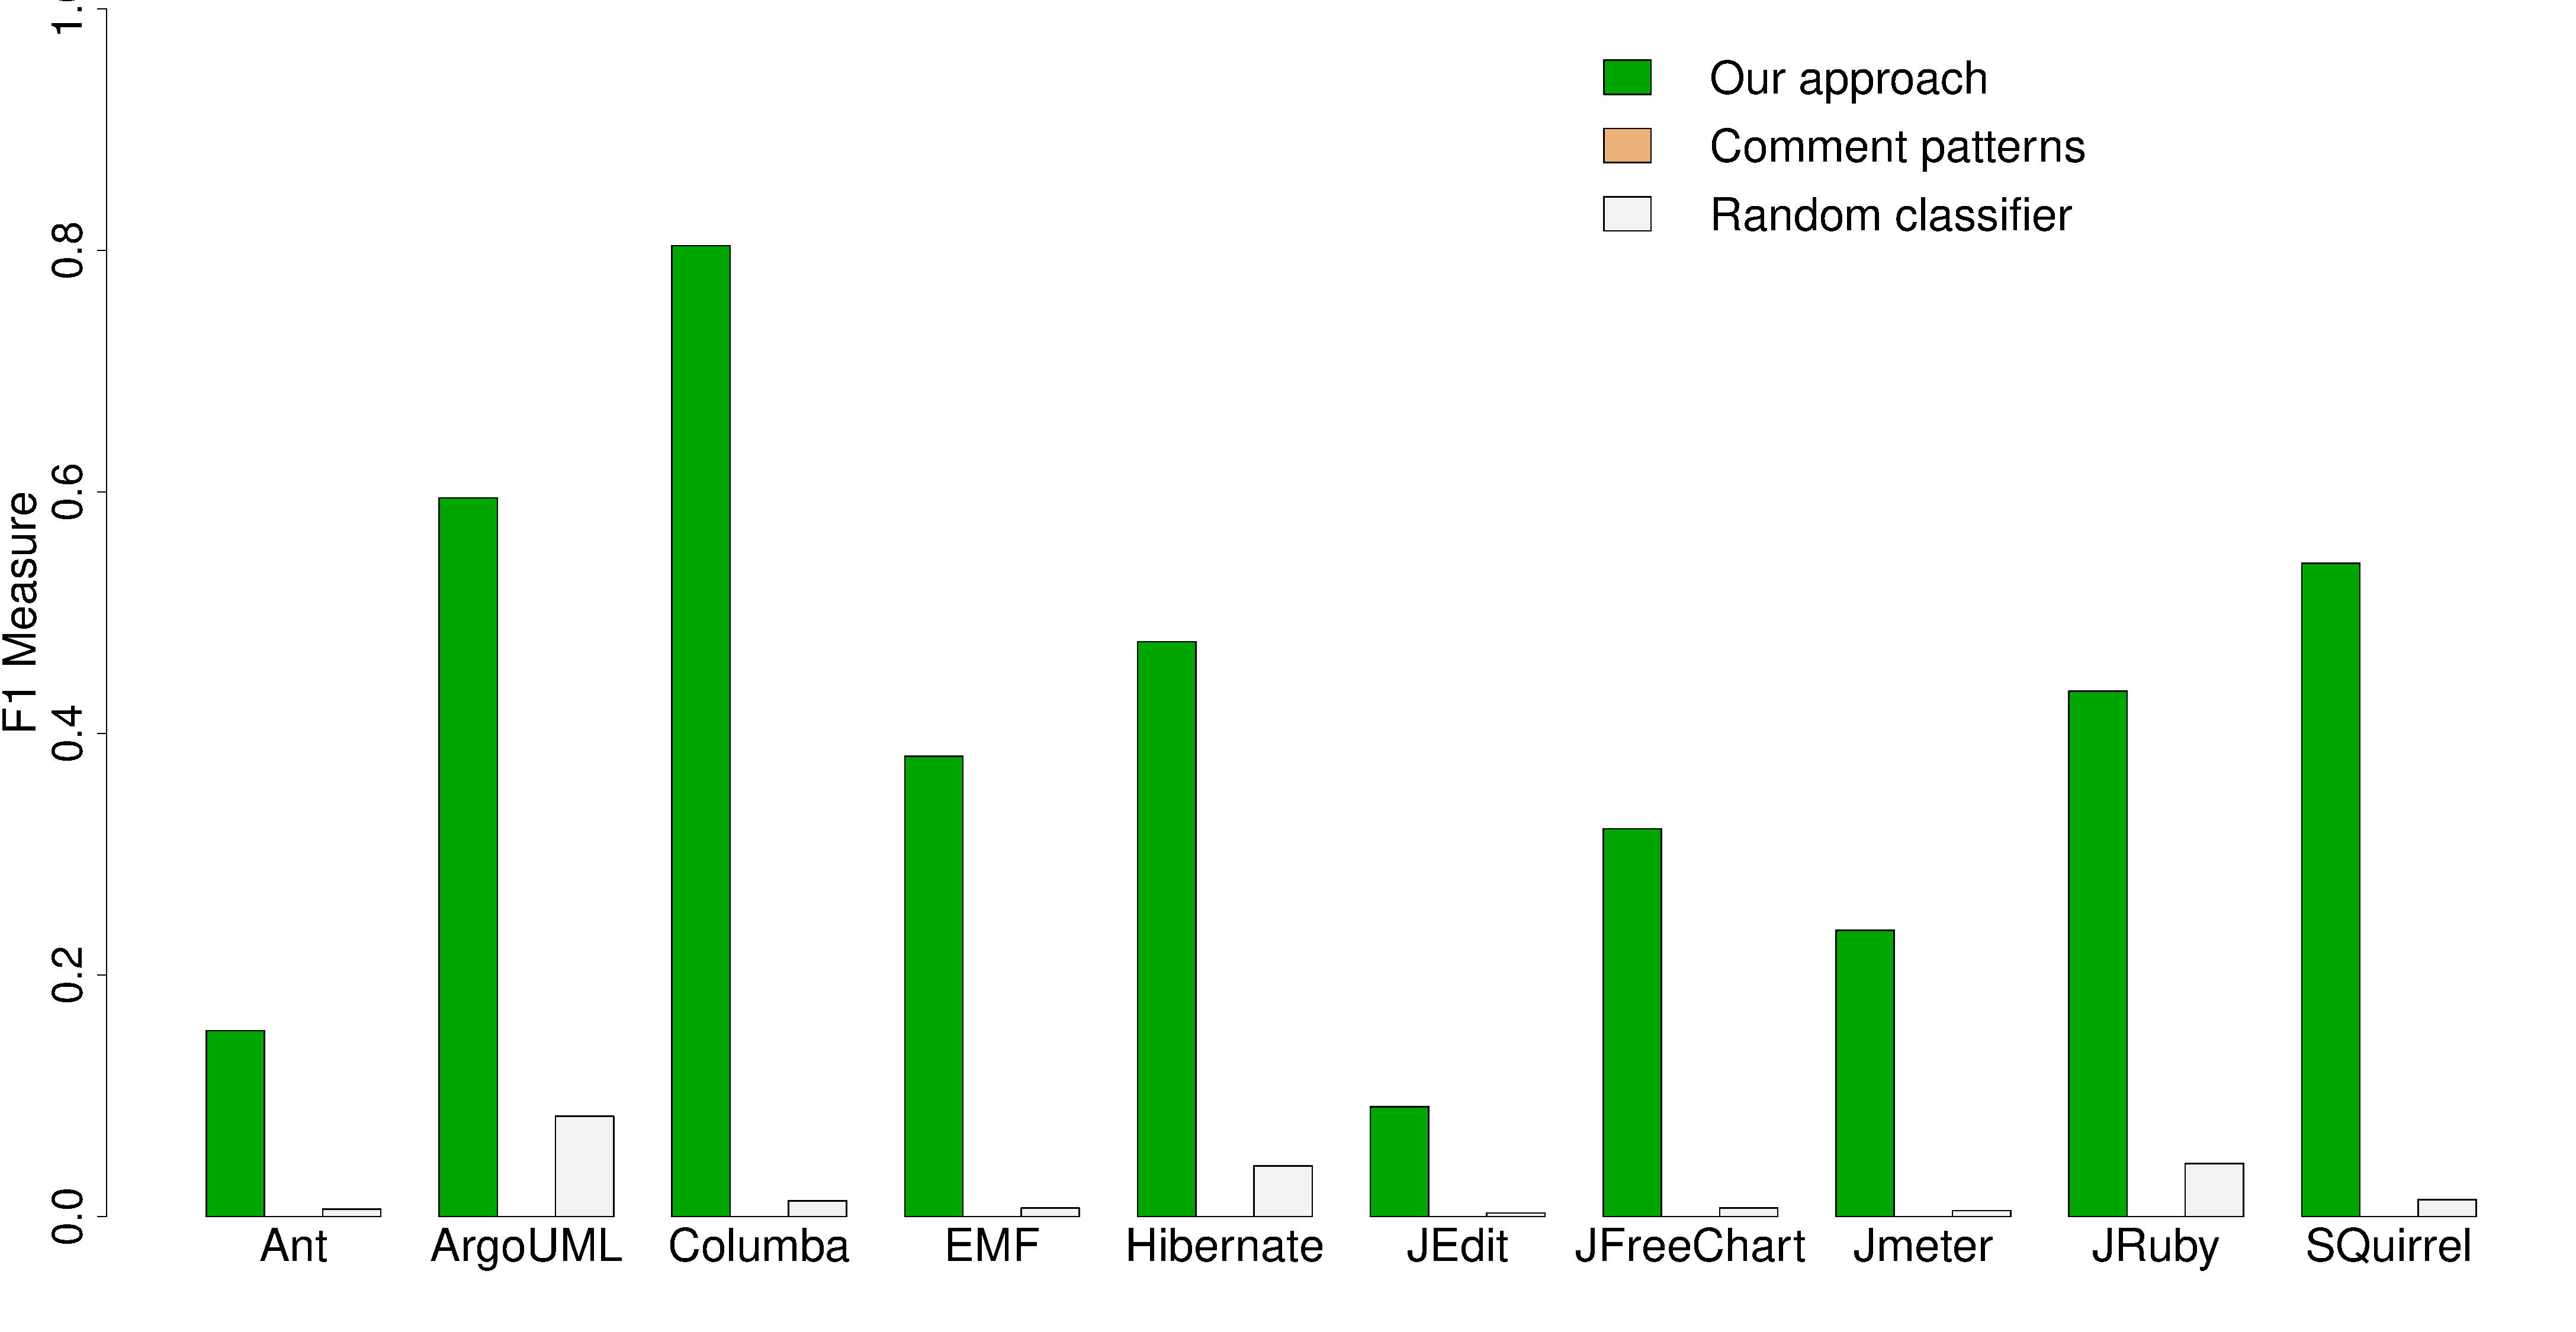
\includegraphics[width=0.4\textwidth]{figures/f1_measure_comparisom_requirement_1.pdf}
  \label{fig:f1_measure_comparison_requirement_debt}}
  \caption{F1 measure comparison}
\end{figure*}


\begin{table*}[!thb]
    \begin{center}
        \caption{Improvement over the baselines F1 measure for design and requirement debt}
        \label{tbl:improvement_f1measure}
        \begin{tabular}{l| c c c c c| c c c}
        \toprule
        
        % draw first line. The * centralizes the Project column, then set the total size of columns that we have
        \multirow{4}{*}{\textbf{\thead{Project}}} & \multicolumn{5}{c|}{\textbf{\thead{Design debt}}} & \multicolumn{3}{c}{\textbf{\thead{Requirement debt}}} 
        % indicates that from now on we are filling the content of the next line
        \\ 
        % \cline{2-2}
        \cmidrule{2-9}
        % remainder columns
        & {\textbf{\thead{Our\\approach}}} & {\textbf{\thead{Comment\\patterns}}} & {\textbf{\thead{Random\\classifier}}} & {\textbf{\thead{Improvement over\\comment patterns}}} & {\textbf{\thead{Improvement over\\random classifier}}} & {\textbf{\thead{Our\\approach}}} & {\textbf{\thead{Random\\classifier}}} & {\textbf{\thead{Improvement over\\random classifier}}} \\
  
        \midrule                                                  
        \textbf{Ant}          &  0.517  &  0.175 & 0.045 &  2.9$\times$   &  11.4$\times$  & 0.154  &  0.006  & 25.6$\times$  \\
        \textbf{ArgoUML}      &  0.814  &  0.078 & 0.155 &  10.4$\times$  &  5.2$\times$   & 0.595  &  0.083  & 7.1$\times$   \\
        \textbf{Columba}      &  0.601  &  0.145 & 0.038 &  4.1$\times$   &  15.8$\times$  & 0.804  &  0.013  & 61.8$\times$  \\
        \textbf{EMF}          &  0.470  &  0.114 & 0.035 &  4.1$\times$   &  13.4$\times$  & 0.381  &  0.007  & 54.4$\times$  \\
        \textbf{Hibernate}    &  0.744  &   0.15 & 0.214 &  4.9$\times$   &  3.4$\times$   & 0.476  &  0.042  & 11.3$\times$  \\
        \textbf{JEdit}        &  0.509  &  0.324 & 0.037 &  1.5$\times$   &  13.7$\times$  & 0.091  &  0.003  & 30.3$\times$  \\
        \textbf{JFreeChart}   &  0.492  &  0.053 &  0.08 &  9.2$\times$   &  6.1$\times$   & 0.321  &  0.007  & 45.8$\times$  \\
        \textbf{Jmeter}       &  0.731  &  0.127 & 0.075 &  5.7$\times$   &  9.7$\times$   & 0.237  &  0.005  & 47.4$\times$  \\
        \textbf{JRuby}        &  0.783  &  0.138 & 0.131 &  5.6$\times$   &  5.9$\times$   & 0.435  &  0.044  & 9.8$\times$   \\
        \textbf{SQuirrel}     &  0.540  &  0.071 & 0.056 &  7.6$\times$   &  9.6$\times$   & 0.541  &  0.014  & 38.6$\times$  \\
        \midrule 
        \textbf{Average}      &  0.620  & 0.137 & 0.086 &   4.5$\times$   & 7.1$\times$     & 0.403  &  0.022  & 18$\times$  \\ 
        \bottomrule
        \end{tabular}
    \end{center}    
\end{table*}

\vspace{3mm}
\noindent\rqi
\vspace{3mm}

\noindent \textbf{Motivation:} As shown in previous work \cite{Potdar2014ICSME, Maldonado2015MTD}, \SATD comments can be found in the source code. However, there is no automatic way to identify these technical debt comments. The methods proposed so far heavily rely on manual examination of source code, and there is no evidence on how well these approaches perform. Moreover, the state-of-the-art approaches to detect \SATD do not discriminate between the different types of technical debt (e.g., design, test, requirements).

Therefore, we want to determine if NLP tools such as, the Stanford NLP Classifier, can help us to surpass these limitations. NLP tools can automatically classify comments based on specific linguistic characteristics of these comments. Answering this question is important, since it helps us understand the opportunities and limitations of using NLP techniques to automatically identify \SATD comments. 

%These characteristics are obtained through the training dataset that we created. 

%For example, the training dataset can show that the adjective `ugly' is frequently found in \SATD comments. 

\vspace{1mm}
\noindent \textbf{Approach:} In this RQ, we would like to examine how effectively we can identify design and requirement \SATD. Therefore, the first step is to create a dataset that we can train and test our NLP classifier on. We classified the source code comments into the following types of \SATD: design debt, defect debt, documentation debt, requirement debt and test debt. However, our previous work showed that the most frequent \SATD comments are design and requirement debt. Therefore, in this paper, we focus our attention on the identification of these two types of \SATD. We decided to focus on these two types of \SATD since 1) they are the most common types of technical debt and 2) NLP-based techniques require sufficient data for training (i.e., they cannot build an accurate model with a small number of samples).

%As described in Section \ref{sec:approach}, in a combined effort between this work and our previous study on \SATD \cite{Maldonado2015MTD} we manually classify comments from ten open source projects. 

We train the NLP classifier using our manually created dataset. The dataset contains comments with and without \SATD, and each comment contains its own classification (i.e., without technical debt, design debt or requirement debt). Then, we add to the training dataset all comments classified as without technical debt and the comments classified as the specific type of \SATD that we want to detect/predict. We use comments from 9 out of 10 projects that we analyzed to create the training dataset. The comments from the remaining one project are used to evaluate the classification performed by the NLP tool. We choose to create the training dataset using comments from 9 out of 10 projects since we want to train the NLP tool with the most diverse data possible (i.e., comments from different domains of applications). However, we discuss the implications of using different sizes of training data in RQ3. We repeat this process for each of the ten projects, each time training on 9 projects and testing on the remaining 1 project.

Based on the training dataset, the NLP tool will classify each comment in the test dataset. The resulting classification is compared with the manual classification provided in the test dataset and evaluated. If a comment in the test dataset has the same classification as the classification suggested by the NLP tool, we will have a true positive (tp) or a true negative (tn). \everton{True positives are the cases where the NLP tool correctly identifies \SATD comments, and true negatives are comments irrelevant to technical debt that are classified as without technical debt.} Similarly, when the classification provided by the tool diverges from the manual classification provided in the test dataset, we have false positives or false negatives. False positives (fp) are comments classified as being \SATD when they are not, and false negatives (fn) are comments classified as without technical debt when they really are \SATD comments. Using the tp, tn, fp, and fn, we are able to evaluate the performance of different detection approaches in terms of precision (i.e., $\frac{tp}{tp + fp}$), recall (i.e., $\frac{tp}{tp + fn}$) and F1 measure (i.e., $2 \times \frac{P \times R}{P + R}$). To determine how effective the NLP classification is, we compare its F1 measure with the F1 measure of two other approaches. We use the F1 measure to compare the performance between the approaches as this measurement provides the harmonic mean of precision and recall. Using the F1 measure allows us to incorporate the tradeoff between precision and recall and present one value that evaluates both measures.

The first approach is the current state-of-the-art in detection of \SATD comments devised by Potdar and Shihab~\cite{Potdar2014ICSME}. This approach uses 62 comment patterns (i.e., keywords and phrases) that were noticed as recurrent in \SATD comments during the manual inspection of 101,762 comments. The second approach is a simple (random) baseline, which assumes that the detection of \SATD is random. The precision of this approach is calculated by taking the total number of \SATD over the total number of comments of each project. For example, Ant has 4,137 comments, of those, only 95 comments are design \SATD. The chance of randomly finding a design \SATD comment is 0.022 (i.e., $\frac{95}{4,137}$). Similarly, to calculate the recall we take into consideration the two possible classifications available: one is the type of \SATD (e.g., design) and the other is without technical debt. Therefore, there is a 50\% chance that the comment will be a \SATD. 

\vspace{1mm}

\noindent \textbf{Results - design debt:} Table \ref{tbl:improvement_f1measure} presents the F1 measure of the three approaches, as well as the improvement achieved by our approach compared to the two other approaches. We see that for all the projects, the F1 measure achieved by our approach is higher than the other baseline F1 measures. The F1 measure obtained by our NLP-based approach ranges between 0.470 - 0.814, with an average of 0.620. In comparison, the F1 measure using the comment patterns ranges between 0.071 - 0.324, with an average of 0.137, and the simple (random) baseline classifier achieves F1 measures in the range of 0.035 - 0.214, with an average of 0.086. Figure \ref{fig:f1_measure_comparison_design_debt} visualizes the comparison of the F1 measure for our approach, the comment patterns approach and the simple (random) baseline classifier. We see from both, Table \ref{tbl:improvement_f1measure} and Figure \ref{fig:f1_measure_comparison_design_debt} that on average, our approach to identify design \SATD outperforms, the state-of-the-art comment pattern approach by 4.5 times and the simple (random) baseline approach by a factor of 7.1 times. 

It is important to note that each one of the selected baselines for comparison has one strong point. The comment patterns approach has a high precision, but it lacks recall, i.e., this approach points correctly to \SATD comments, but as the approach depends on keywords, it identifies a very small subset of all the \SATD comments in the project.
\nikos{The strong point of the random classifier has been commented out}

%The less sophisticated random classifier baseline provides a high recall because we try to classify comments between two categories (i.e with or without technical debt), meaning a 50\% chance to randomly get one of the two classifications. 

%The second, third and fourth columns of Table \ref{tbl:improvement_f1measure} shows our approach F1 measure, the comment patterns baseline F1 measure and the random classifier baseline F1 measure respectively for each project while classifying design \SATD. In addition, fifth and sixth columns present how many times our approach surpass the comment patterns baseline and the random classifier baseline.   
 
\noindent \textbf{Results - requirement debt:}  The last three columns of Table \ref{tbl:improvement_f1measure} present the performance of our approach, the performance of the simple (random) baseline approach, and the improvement of our approach over the simple (random) baseline. The comment patterns approach was not able to identify any requirement \SATD, hence we omit the presentation of its results. For all projects, the F1 measure obtained by our approach surpasses the simple (random) baseline classifier. Our approach achieves a F1 measure between 0.091 - 0.804 with an average of 0.403, whereas the simple (random) baseline achieves F1 measure in the range of 0.003 - 0.083, with an average of 0.022. Figure \ref{fig:f1_measure_comparison_requirement_debt} visualizes the performance comparison of the two approaches.

Generally, it is clear that requirement \SATD is less common than design \SATD, which makes it more difficult to detect. That said, our NLP-base approach provides a significant improvement over the simple (random) baseline approach, with an average improvement of 18 times.

%Despite the fact that this number is slightly lower than the average obtained while identifying design debt, the quantity of requirement \SATD comments that are present in the projects is very small, which makes its classification more difficult. For example, JEdit has 14 requirement \SATD comments distributed over a total of 10,080 comments (i.e, requirement debt comments plus without \SATD comments). Nevertheless, our approach can identify \SATD even in this unbalanced dataset as we still outperform the random classifier baseline F1 measured by 30.3 times, i.e., the random classifier baseline F1 measure was of 0.003 for JEdit. 

%highest F1 measure was obtained for Columba project with 0.804, and the lowest value was of 0.091 on JEdit. Although there was a big fluctuation between the maximum and minimum value obtained our average F1 measure was of 0.403. 

%Similarly, Figure \ref{fig:f1_measure_comparison_requirement_debt} shows the comparison between the three F1 measures while identifying requirement \SATD.

%We find that the comment patterns approach is not an appropriate approach for identifying requirement \SATD, since it was not able to identify any of the requirement \SATD comments in our analyzed projects. Therefore, we use only the random classifier baseline to compare with our results.

%The seventh column Table \ref{tbl:improvement_f1measure} shows the F1 measure of our approach, the eighth column presents the random classifier baseline F1 measure, and the ninth column shows the improvement of our approach over the random classifier baseline. For example, on SQuirrel project the F1 measure was of 0.541 whereas the random classifier baseline F1 measure was of 0.014, which means that there was an improvement of 38.6 times in the identification of requirement \SATD comments using our approach. 

% The eighth column of Table \ref{tbl:improvement_f1measure} shows the improvement of our approach over the random classifier baseline. For example, on SQuirrel project the F1 measure was of 0.875 whereas the random classifier baseline F1 measure was of 0.04, which means that there was an improvement of 21.8 times in the identification of requirement \SATD comments using our approach. 

\conclusionbox{We find that our NLP-based approach, is more effective in identifying \SATD comments compared to the the current state-of-art approaches. We achieved an average F1 measure of 0.620 when identifying design debt (an average improvement of 4.5$\times$ and 7.1$\times$ compared to other approaches) and an average F1 measure of 0.403 when identifying requirement debt (an average improvement of 18$\times$).}

\vspace{3mm}
\noindent\rqii
\vspace{3mm}

\noindent \textbf{Motivation:} After asserting the efficiency of our NLP-based approach in identifying \SATD comments we want to better understand what words developers use when indicating this technical debt. Answering this question will provide insightful information that can guide future research directions, broaden our understanding on \SATD and also help us to detect it.     

\vspace{1mm}
\noindent \textbf{Approach:} To perform its detection, the NLP tool learns optimal features that can be used to detect \SATD. These features, are fragments of data (e.g., words) that are associated with a specific type of debt (e.g., design debt, requirement debt, or without technical debt). Moreover, each feature has a weight, which represents how strongly the feature relates to a specific type of debt. The NLP tool uses the labeled training data that we input to determine the features and their weigh. Then, the features and their corresponding weights are used to determine if a comment belongs to a specific type of \SATD.

For example, if the NLP tool, based on the training data, determines that the two features ``hack'' and ``dirty'' are related to design debt with weight 5.3 and 3.2, respectively, and the feature ``something'' relates to the non-technical debt class with a weight of 4.1. Then, if we aim to classify the comment ``this is a dirty hack it's better do to something'' in our test data, all features will be analyzed and the following score would be calculated design debt weight = 8.5 (i.e., feature `hack' weight plus feature `dirty' weight) and without technical debt weight = 4.1 resulting in a comment classified as design debt.

%The features are extracted from the comments in the training dataset, and then applied to the test dataset where they are combined to reach a vote. That is, every feature that is satisfied by the comment being classified (i.e., matched) will be used to predict the class for the comment. The vote is given to the class with highest weight. 

For each analyzed project, we collect the features used to predict the \SATD comments. These features are provided by the NLP tool as output and stored in a text file. The features are written in the file based on the weight that they have, ordered by highest weight to the lowest weight, meaning more relevant features to less relevant features respectively. Based on these files, we rank the words calculating the average ranking position of the analyzed feature across the ten different projects. 

%We determined the top 10 features (i.e, most relevant based on the weight) for design and requirement \SATD comments.

\noindent \textbf{Results:} Table \ref{tbl:top_ten_features} shows the top 10 textual features used to identify  \SATD in the ten studied projects, ordered by their weight \emad{relevance or weight?}. The first column we present the ranking of each textual feature, the second column lists the features used in the identification of \emph{design} \SATD, and the third column lists the textual features used to identify \emph{requirement} \SATD.

\begin{table}[!thb]
    \begin{center}
        \caption{Top Ten Textual Features Used to Identify Design and Requirement Self-Admitted Technical Debt}
        \label{tbl:top_ten_features}
        \begin{tabular}{l| l l }
        \toprule
        \textbf{Rank} & \textbf{Design Debt} & \textbf{Requirement Debt}  \\
        \midrule
         1  & hack       &   todo              \\
         2  & workaround &   needed            \\
         3  & yuck!      &   implementation    \\
         4  & kludge     &   fixme             \\
         5  & stupidity  &   xxx               \\
         6  & needed?    &   ends?             \\
         7  & columns?   &   convention        \\
         8  & unused?    &   configurable      \\
         9  & wtf?       &   apparently        \\
         10 & todo       &   fudging           \\
        \bottomrule
        \end{tabular}
    \end{center}    
\end{table}

From Table~\ref{tbl:top_ten_features} we observe that top ranked textual features, i.e., hack, workaround, yuck!, kludge and stupidity, are related to design \SATD indicate sloppy or mediocre source code. Other textual features such as needed?, columns?, unused?, wtf? and todo, are questioning the usefulness or utility of specific source code. For requirement \SATD, the top ranked features, i.e., todo, needed, implementation, and fixme, indicate the need to enhance or complete the implementation in the future. Other lower ranked textual features such as xxx, ends?, convention, configurable, apparently and fudging, indicates potential future enhancements that make the code more configurable and/or generic. \emad{not sure if I am using the right words here - maybe even add 1 or 2 examples here}

We also observe that it is possible a single textual feature to indicate both design and requirement \SATD. However, in such cases, the ranking of the textual features for design and requirement \SATD is different. For example, the work todo is ranked tenth for design debt, whereas it is ranked first for requirement debt. This finding is intuitive, since requirement debt will naturally be related to the implementation of future functionality.

It is important to note here that although we present the top 10 textual features, the classification of the comments is based on a combination of several textual features. In fact, on average, the number of features used to classify design debt is 6,196 and 2,889 for requirement debt. The exact number of unique textual features used to detect \SATD for each project is shown in Table \emad{Everton add table}. The fact that our NLP-based approach leverages so many features helps to explain the significant improvement we are able to achieve over the state-of-the-art~\cite{Potdar2014ICSME}, which only uses 62 patterns that are composed of \todo{X} unique textual features.

%This shows why our recall is much better than Potdar and Shihab's ~\cite{Potdar2014ICSME}. 

\conclusionbox{We find the that design and requirement debt have their own textual features that best indicate such \SATD comments. For design debt, the best indicative textual features indicate sloppy or mediocre source code, whereas for requirement debt they relate to the need to enhance or complete the implementation in the future.}

\vspace{3mm}
\noindent\rqiii
\vspace{3mm}

\noindent \textbf{Motivation:} Thus far, we have shown that our NLP-based approach can effectively identify \SATD comments. However, we conjuncture that the performance of the classification depends on the amount of training data. At the same time, creating the training dataset is expensive and manually intensive. So, the question that arises is: how much training data do we need to effectively classify the \SATD comments? If we need a high number of comments to create our training dataset, our approach will be more difficult to extend and applied for other projects. On the other hand, if a small dataset can be used to identify \SATD comments, then this approach can be applied with minimal effort, i.e., less training data. That said, intuitively we expect that the performance of the classifier would improve as more comments are being added to the training dataset.


\noindent \textbf{Approach:} To answer our research question, we followed a systematic process where we incrementally add training data and evaluate the performance of the classification. Since we have 10 projects in our dataset, we use one project as testing data, and the remaining nine projects to train. However, we do not train the classifier with all nine projects, instead, we add each project incrementally. We repeated this process for each project and report on our findings.

%We executed the classification process several times with an increasing number of comments being added to the training dataset while collecting the results to analyze the changes between each iteration.

%We first select a project that will be classified by the Stanford Classifier.

%Second, with one of the remainder projects, we select all \SATD comments (i.e., design or requirement debt accordingly with what we want to classify), and all comments without technical debt as well. These comments are added to the training dataset and fed into the Standford Classifier. Then, the results of the classification are collected and stored for analysis.

%Third, the comments of other project is added to the training dataset and the results of the classification are collected once more. The order that projects are added to the training dataset is not random. We add first projects which has more \SATD comments of the specific type that we are trying to identify. We cycle through the above steps until we had added the comments of all nine projects to the training dataset.

%Fourth, we select another project to be classified by the Stanford Classifier, and we repeat this process until we have analyzed all our projects.

To determine how much data is required to effectively identify \SATD comments, we compute the F1-measure after each iteration (an iteration is simply a run with a different size of training data). We record the iteration that achieves the highest F1-measure and the number of projects used in the training dataset to achieve this F1-measure. Then, we record the number of projects needed to achieve at least 90\% and 80\% of the maximum F1-measure.
%Based on the maximum F1 measure we calculate how close the others iterations were from achieving the same value.

For example, if the maximum F1-measure is 0.85 and it is achieved in the 8th iteration (i.e., using 8 projects in the training dataset), and during the 4th iteration we achieve a F1-measure of 0.80, then we say that we can achieve at least 90\% (94\% to be exact) of the maximum F1-measure with a training dataset constructed from just 4 projects. Since the results will differ for the different projects, we repeat this analysis for all projects and present the average F1-measures across all projects.
% Once the percentage of the maximum F1 measure is calculated for all iterations we analyze the quantity of comments used in the training dataset by them.

\begin{figure}[t]
  \centering
  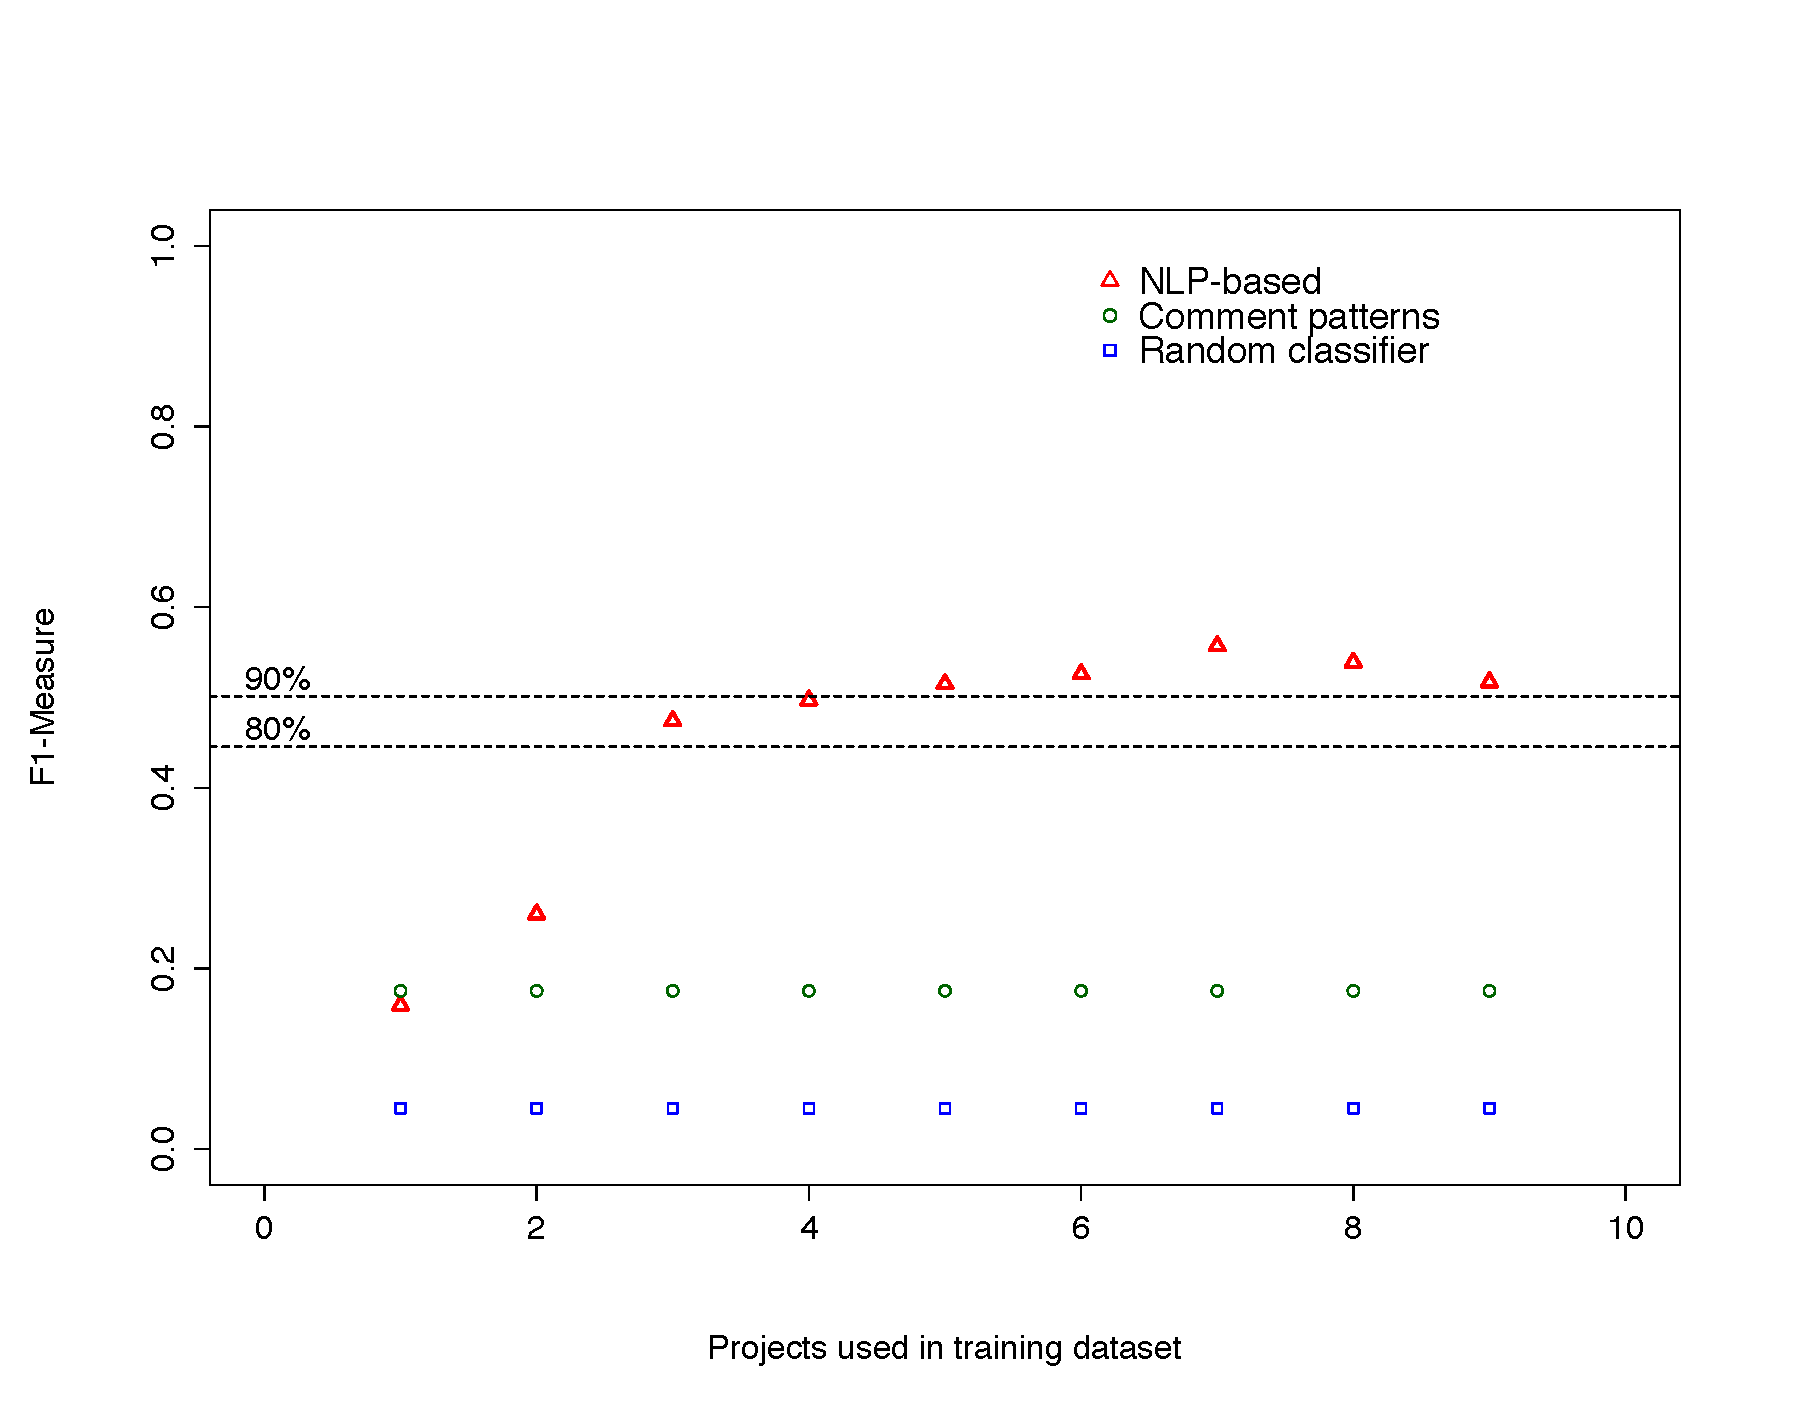
\includegraphics[width = 0.48\textwidth]{figures/design_ant.pdf}
  \vspace{-3mm}
  \caption{Ant Design Debt classification}
  \label{fig:design_ant_result}
\end{figure}

\begin{figure}[t]
  \centering
  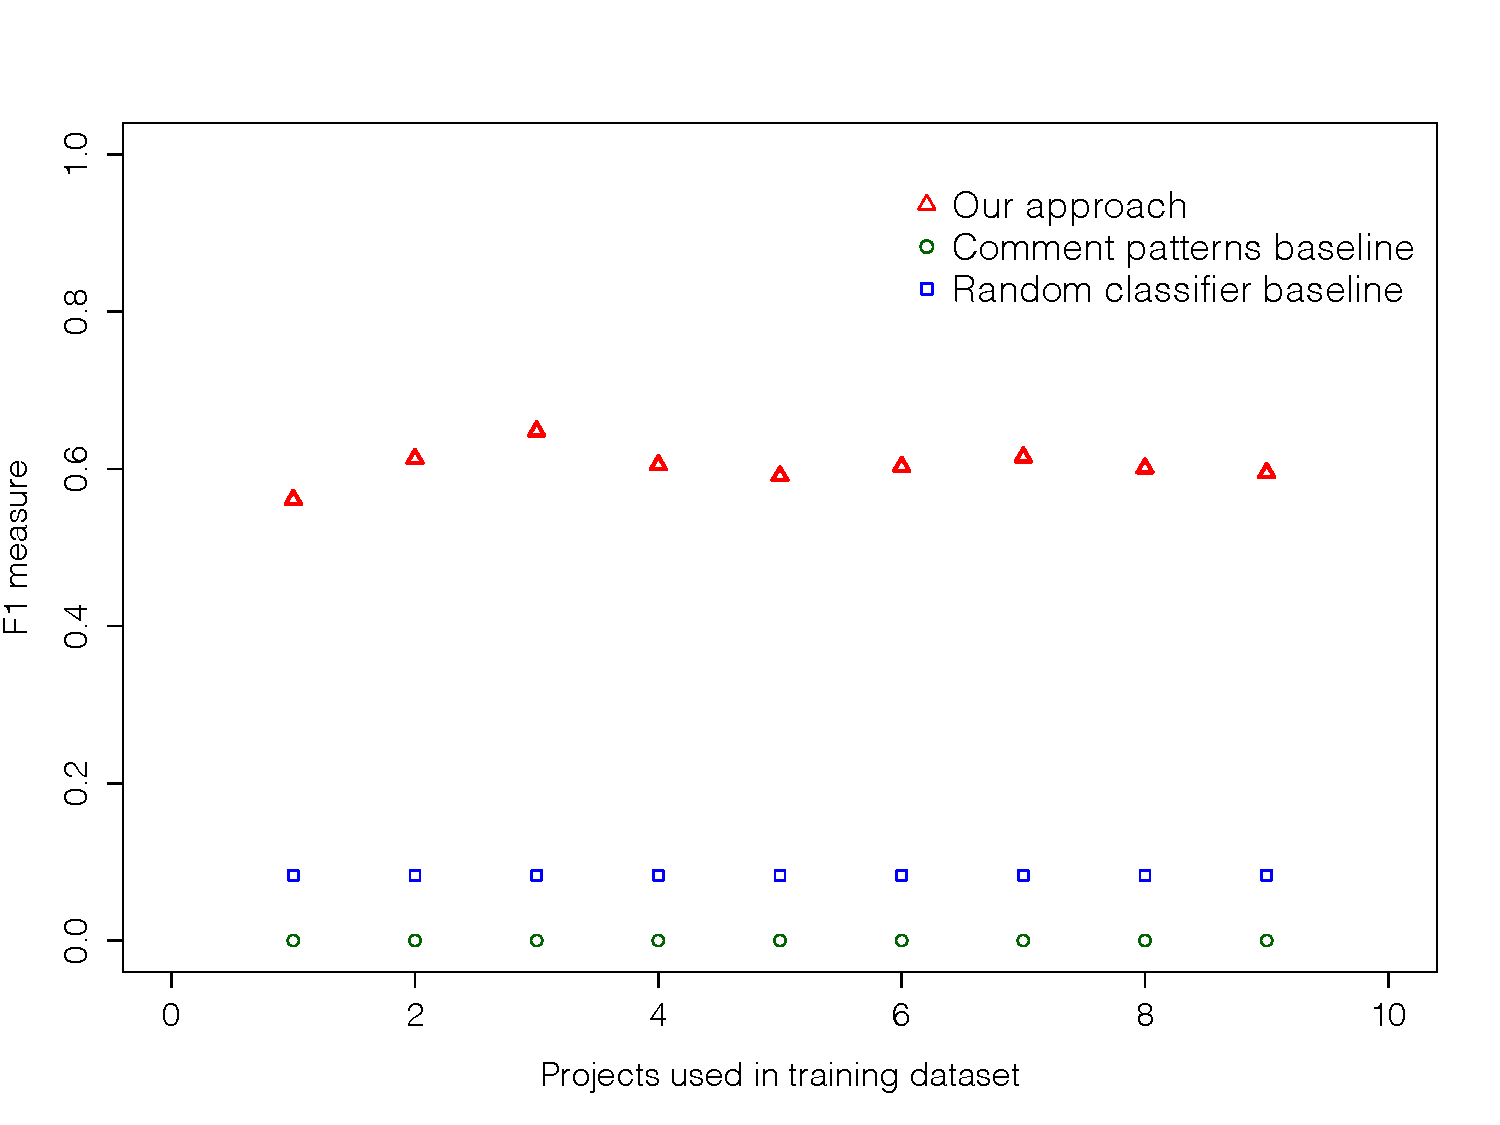
\includegraphics[width = 0.48\textwidth]{figures/implementation_argo}
  \vspace{-3mm}
  \caption{ArgoUml Requirement Debt classification}
  \label{fig:implementation_argo_result}
\end{figure}

%Therefore, we determined which iteration has the highest performance for each project. We called this iteration as the maximum F1 measure. To know how close the other iterations were from reaching the maximum performance we use the iteration F1 measure value to calculate the percentage of the maximum F1 measure that it represents. We calculate these values for design and requirement debt separately.

\noindent \textbf{Results - design debt:}  Figure~\ref{fig:design_ant_result} shows the F1-measure using different sizes of training data for the Ant project. Due to space, we discuss the results for a representative project (Ant) in this section, however, figures for all projects are provided in the Appendix \todo{add}. From Figure~\ref{fig:design_ant_result}, we find that the maximum F1-measure improves as we increase the number of projects (i.e., iterations), achieving the highest F1-measure in the seventh iteration and slightly decreasing afterwards. The horizontal lines in the figure show the 90\% and 80\% of the highest F1-measure. We can see from Figure~\ref{fig:design_ant_result} that with \todo{1,499 comments (i.e., from 3 projects)} and \todo{x}, we can achieve 90\% and 80\% of the highest F1-measure, respectively. This amounts to a reduction of \todo{X\%} in training data to achieve 90\% and 80\% of the maximum F1-measure, respectively. Considering the tradeoff in accuracy versus the amount of training data, for Ant, using only \todo{3} or \todo{4} projects provides the best tradeoff.

%The three highest values of the F1 measure in Figure \ref{fig:design_ant_result} are: 0.526, 0.539 and 0.557 obtained during the 6th, 8th and the 7th iteration respectively.

\emad{Everton, copy the correct results from the commented out paragraph here. Also add the horizontal lines to the figures.}
%We notice that in the 3rd iteration the F1 measure was 0.474, and the maximum F1 measure achieved for the project (i.e., 7th iteration) was 0.557. The F1 measure achieved in the 3rd iteration represents 85\% of the maximum F1 measure achieved in the 7th iteration, and this percentage was reached using 1,499 comments (i.e., from 3 projects) whereas the maximum F1 measure used 2,404 comments (i.e., from 7 projects) in the training dataset. Therefore, for Ant we could achieve 85\% of the maximum result using only 62\% of the comments. We argue that the third iteration provides a good tradeoff between prediction performance and number of comments used to create the training dataset.

Because the results differ for different projects, we also analyzed the \todo{iterations projects}\nikos{there is something wrong in the wording here. This paragraph is hard to understand} to determine the iterations that achieve the best performance across all projects. To measure that, we calculate the average percentage of the maximum F1 measure for each iteration. For example, we take the average percentage of the maximum F1 measure achieved during the 1st iteration for all projects, then we calculate the same value for all 2nd iterations and so on. We find that, the best performance is achieved during the 8th iteration, with an average maximum F1-measure of 96.57\% using (on average) 2,353 comments to create the training dataset. In comparison, the 9th iteration has an average  maximum F1-measure of 95.99\%, which is slightly lower than the average obtained in the 8th iteration, and uses more comments in the training dataset (i.e., 2,432). 
%As mentioned before, the addition of more comments not necessary implies more performance.

Table \ref{tbl:design_iteration_performance} shows the average percentage of the maximum F1-measure for each iteration. The first column shows the iteration number. The second column shows the average percentage of the maximum F1-measure achieved for each iteration. The third column presents the delta interval of the average percentage of the maximum F1-measure between one iteration and the previous one. The fourth column shows the average number of comments used in the training dataset of that specific iteration. Table \ref{tbl:design_iteration_performance} shows that, on average, we can achieve more than 90\% and 80\% of the maximum F1-measure in the second and third iterations, respectively. To achieve more than 90\% and 80\% of the maximum F1-measure, we require 1,444 (64.14\% of total comments required in 7th iteration) and 1,106 (49.13\% of total comments required in 7th iteration) comments, respectively.\nikos{I think it should be ``more than 80\% and 90\% of the maximum...'' in both cases. reverse the percentages}

\noindent \textbf{Results - requirement debt:} We find that although there is a variation in the F1 measure value during the first 3 iterations, they are not as preeminent as the variation found in design \SATD analysis. The F1 measure in requirement \SATD tends to be more constant through the iterations, and the first iteration has already a high percentage of the maximum F1 measured achieved for each project. This shows that the way the developers indicate requirement debt does not vary between different application domains as much as in design debt. This uniformity in requirement \SATD comments allows a good classification even with a small number of comments in the training dataset. We elaborate more on this point later in Section~\ref{sec:discussion}.

Figure \ref{fig:implementation_argo_result} \emad{check the figure ref...seems wrong} shows the F1-measure for different iterations in ArgoUML. The highest F1-measure of 0.65 \emad {use 2 decimal points throughout the paper} is achieved in the third iteration. From Figure~\ref{fig:implementation_argo_result}, we observe that we achieve more than 90\% and 80\% of the highest F1-measure in iterations \todo{x} and \todo{y}, respectively. The reduction in comments is \todo{add result} for the 90\% and 80\% of the maximum F1-measure, respectively.

%ArgoUML presented small increases in F1-measure during the first three iterations reaching the best result at the 3rd iteration, 0.648. However, there was low variation in the F1 measure performance between iterations 4th (0.605) to 9th (0.595). In the 1st iteration (0.561) the classifier was trained with 110 requirement \SATD comments, which means 31\% of the comments that where used in the 9th iteration (0.595). A reduction of 69\% of the necessary training data to achieve almost the same result in terms of F1 measure in this case. 

Table \ref{tbl:requirement_iteration_performance} shows the average percentage of the maximum F1-measure for each iteration. Unlike the case of design debt, for requirement debt, the best F1-measure is achieved in the first iteration. This shows that using as few as 380 comments, we can effectively detect requirement \SATD.

%, the delta interval of the average maximum F1 measure between each iteration and the average number of comments used to create the training dataset. We also analyzed the average percentage of the maximum F1 measure between all iterations across the projects. We find that the 1st iteration was the one with the highest average percentage of the maximum F1 measure achieving a value of 87.3\% followed by the 7th iteration, with 83.7\% of the maximum F1 measure. The training dataset of the 1st iteration sized, on average, 380 \SATD comments. In comparison, an average of 654 requirement \SATD comments were used in the training dataset representing 97\% of all requirement \SATD comments that we classified during this study. This means that the 1st iteration, on average, performed better than the other iterations using only 55\% of the available training dataset at our disposal.

\begin{table}[!thb]
    \begin{center}
        \caption{Average maximum F1 measure for Design Debt  for all projects}
        \label{tbl:design_iteration_performance}
        \begin{tabular}{l| c c c}
        \toprule
        \thead{Iteration\\Number} & \thead{Average\%\\of maximum\\F1 measure} & \thead{$\Delta$\\between\\iterations} & \thead{Average\\comments} \\
        \midrule
         1  &  0.718 &  -      & 756   \\  
         2  &  0.856 & 0.138   & 1,106 \\  
         3  &  0.924 & 0.068   & 1,444 \\  
         4  &  0.912 & -0.012  & 1,717 \\  
         5  &  0.927 & 0.016   & 1,919 \\  
         6  &  0.930 & 0.002   & 2,108 \\  
         7  &  0.963 & 0.029   & 2,251 \\  
         8  &  0.965 & 0.006   & 2,353 \\  
         9  &  0.959 & -0.002  & 2,432 \\  
        \bottomrule
        \end{tabular}
    \end{center}    
\end{table}

\begin{table}[!thb]
	\begin{center}
		\caption{Average maximum F1 measure for Requirement Debt for all projects}
		\label{tbl:requirement_iteration_performance}
		\begin{tabular}{l| c c c}
			\toprule
			\thead{Iteration\\Number} & \thead{Average\%\\of maximum\\F1 measure} & \thead{$\Delta$\\between\\iterations} & \thead{Average\\comments} \\
			\midrule
			1  &  0.873 &   -      &  380 \\  
      2  &  0.772 & -0.101   &  481 \\
      3  &  0.778 & 0.006    &  541 \\  
      4  &  0.806 & 0.028    &  588 \\
      5  &  0.795 & -0.011   &  620  \\
      6  &  0.819 & 0.024    &  638  \\
			7  &  0.837 & 0.018    &  654  \\  
      8  &  0.833 & -0.004   &  668  \\  
      9  &  0.805 & -0.028   &  681  \\  
			\bottomrule
		\end{tabular}
	\end{center}    
\end{table}

%It is important to notice that, this results shows that it is possible to identify \SATD with a lower number of comments. Using a lower number of comments to create the training dataset makes the approach more applicable as the number of \SATD comments is rather scarce.    

The results of this RQ show that, contrary to our initial intuition, more data need not result in higher classification accuracy. In fact, we find that in some cases, the addition of more comments can decrease the performance of the classifier. One of the reasons for this is that the weight of features is given through empirical probability, and consequently features that appear more will have a higher weight. Although this is an effective process for the majority of the cases we studied, it can be misleading when classifying comments that have different contexts, i.e., in cross-project classification.

\conclusionbox{We find that using our NLP-based approach, design \SATD comments can be classified effectively using a training dataset of 1,106 - 1,444 comments. Similarly, requirement \SATD can be classified with as little as 380 comments of this type.}